%\documentclass[../main.tex]{subfiles}
\setlength{\parindent}{2em}

\chapter{Methodology}
    \section{Dataset Collection}
    \noindent
    Thyroid ultrasound is a safe, non-invasive imaging technique that uses sound waves to create detailed images of the thyroid gland. It helps assess the gland's size, shape, and structure, and detect nodules or abnormalities without the use of radiation, making it a preferred diagnostic tool for thyroid evaluation.
    \par \noindent The benign class encompasses thyroid nodules that are non-cancerous and harmless. These nodules are often curable and do not spread to other parts of the body, requiring minimal or no treatment. On the other hand, the malignant class includes nodules that are suspicious of thyroid cancer. These nodules exhibit characteristics that may indicate malignancy, necessitating further diagnostic tests and timely medical intervention to prevent progression and ensure effective treatment.
    \par \noindent The dataset contains images as per the ‘TIRADS’ score. The classification of thyroid disease is based on the Thyroid Imaging Reporting and Data System (TIRADS) score. This score is calculated using specific parameters, such as nodule composition, echogenicity, shape, margin, and echogenic foci, which help assess the risk of malignancy and guide further diagnostic or treatment decisions.
    

    \subsection{TIRADS}
    \noindent
    The Thyroid Imaging Reporting and Data System (TI-RADS), introduced by the American College of Radiology (ACR) in 2017, is a standardised framework designed to improve the diagnostic accuracy of thyroid nodules and reduce unnecessary biopsies of benign nodules. This system evaluates thyroid nodules based on five key ultrasound features: composition, echogenicity, shape, margin, and punctate echogenic foci. Each feature is assigned a specific point value, which contributes to the overall TI-RADS score. \par \noindent
    \noindent The TI-RADS score categorises nodules into five risk levels: 
    \begin{itemize}
    \item TR1 (0-2 points): Benign – No risk of malignancy.
    \item TR2 (2-3 points): Not suspicious – Likely benign.
    \item TR3 (3-4 points): Mildly suspicious – Low risk of malignancy.
    \item TR4 (4-6 points): Moderately suspicious – Intermediate risk of malignancy.
    \item TR5 (7 or more points): Highly suspicious – High risk of malignancy.
    \end{itemize}

    \noindent
    TI-RADS scores are assigned based on a certain set of features, these features are defined by the American College of Radiology(ACR). The features are identified by radiologists, and in conventional methods, they evaluate those features to give some points based on which a TI-RADS score is given. The figure \ref{fig:tiradsACR} lists all the features defined by ACR and score calculation.

    \begin{figure}[H]
        \centering
        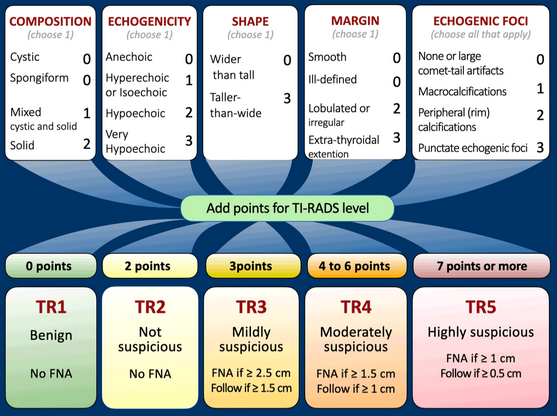
\includegraphics[width=1\linewidth]{images/tiradsACR.png}
        \caption{TIRADS Score}
        \label{fig:tiradsACR}
    \end{figure}

    \noindent
    Based on the TI-RADS score, radiologists determine the need for further diagnostic procedures, such as fine-needle aspiration biopsy (FNAB), to confirm or rule out thyroid cancer. This systematic approach ensures a more accurate and efficient evaluation of thyroid nodules, aiding in timely and appropriate clinical decision-making. \par \noindent
    \noindent The dataset contains multiple samples of different patients’ thyroid glands from different views, which are classified as per the TIRADS score.

    \begin{figure}[ht]
    \centering
    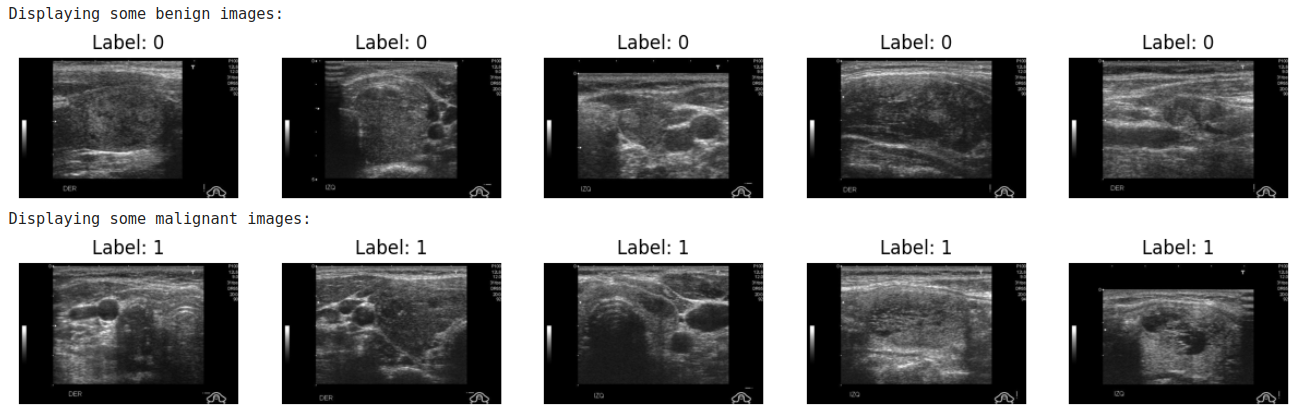
\includegraphics[width=\textwidth]{images/dataset.png}
    \caption{Sample of Ultrasound images from Dataset (0-Benign,1-Malignant).}
    \label{fig:thyroid_nodules}
\end{figure}
    \subsection{Data Preparation}
    \noindent
    All images in the dataset have a resolution of 560x360 pixels and are stored in a 24-bit RGB format (3 dimensions). Before being used as input for the Convolutional Neural Network (CNN), the images undergo preprocessing. This includes converting the images to an 8-bit unsigned integer (uint8) format and transforming them into grayscale, reducing the image to a single dimension. This preprocessing step ensures compatibility with the CNN model and optimises computational efficiency.
    \par \noindent During dataset preparation, the images are categorised into two classes: Benign and Malignant, based on their TI-RADS scores. Specifically, nodules with TR1 and TR2 scores are classified as Benign, as they indicate no or low suspicion of malignancy. On the other hand, nodules with TR3, TR4, and TR5 scores are categorised as Malignant, as TR3 represents mild suspicion, while TR4 and TR5 indicate moderate to high suspicion of malignancy. This classification ensures a clear distinction between benign and potentially cancerous nodules for training the model.
    \par \noindent The dataset is divided into training and testing subsets using the train-test split method. In the current approach, a test size of 0.2 is used, meaning 20\% of the dataset is allocated for testing, while the remaining 80\% is utilised for training the model. This split ensures a balanced distribution of data for evaluating model performance and generalisation.

    \section{CNN Model}
    \noindent
    The Convolutional Neural Network (CNN) is a specialised architecture within the domain of Deep Learning, specifically designed to interpret and analyse visual data. Unlike traditional Artificial Neural Networks (ANNs), which struggle to process raw image data directly, CNNs leverage the convolution operation as a fundamental image processing layer. This operation enables the network to automatically extract spatial features, such as edges, textures, and patterns, from images, making CNNs highly effective for tasks like image classification. By hierarchically learning these features, CNNs can understand complex visual information, outperforming ANNs in tasks involving image data. As a result, CNNs have become the preferred choice for image classification and other computer vision applications. \par \noindent
    The pooling layer plays a crucial role in downsampling the feature maps generated by the convolutional layer, reducing their spatial dimensions while retaining essential information. Following this, the dense layer (fully connected layer), like layers in an Artificial Neural Network (ANN), processes the feature maps. Before being fed into the dense layer, the feature maps are flattened into a 1-dimensional array. The dense layer then interprets these features to produce the final output, typically in the form of class probabilities, enabling the model to make predictions. Figure \ref{fig:CNN} shows the basic flow of the image data across the CNN model. Here, only three layers have been shown, but actual CNN models may contain multiple convolutional and maxpool layer and their multiple configurations. 

    \begin{figure}
        \centering
        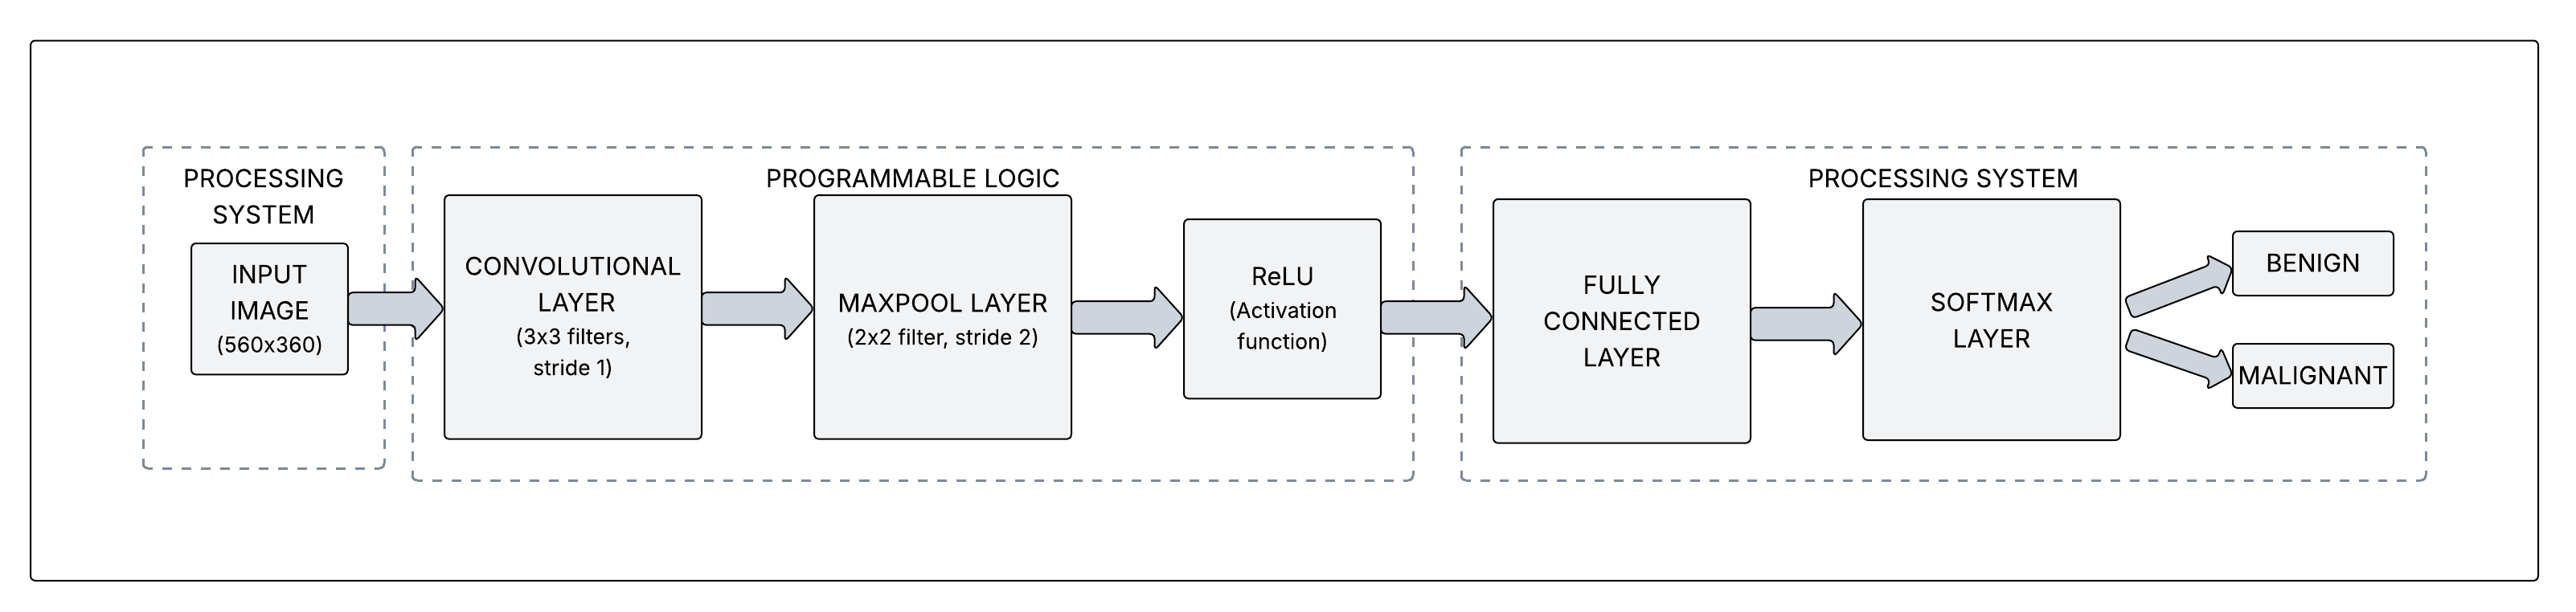
\includegraphics[width=1\linewidth]{images/block diagram overall.png}
        \caption{Overall block diagram}
        \label{fig:overall block diagram}
    \end{figure}

    \section{Hardware Software Partitioning}
    \noindent
    The PYNQ Z2 board belong to the ZYNQ-7000 SoC family of FPGA by Xilinx (now AMD), which integrates the software programmability of an ARM-based dual-core processor with the hardware programmability of an FPGA. The ARM processor is commonly referred to as the PS, whereas the FPGA fabric, where all the LUTs, BRAMs \& DSPs are present, is referred to as PL. There are several interfaces available for the PS and PL to communicate with one another. The PS is programmed in a high-level language like C/C++, and the PL is programmed using HDL languages or Xilinx IP cores, hence PS is known as Software, and the PL is known as Hardware. While designing an accelerated application the application should be partitioned to have maximum benefit from the PS as well as the PL, the PL is very good at performing compute-intensive tasks because of its parallelism capabilities however it performs weakly in tasks which are memory intensive, but the PS can handle the memory intensive tasks very well as compared to the PL. \par \noindent
    The CNN model involves mainly three distinct layers the convolutional layer, the pooling layer and the dense/fully connected layer keeping in mind the points mentioned above the CNN model is partitioned to achieve a better acceleration scheme all three layers are highly compute-intensive but the convolutional layer and pooling layer are very less memory intensive, the convolutional layer involves only a few amounts of weights biases which need to be stored on the PL and the pooling layer has no weights and bias associated to it thus this fact makes them suitable for the implementation of these layers on PL while the fully connected layer consists of a large number of weights and biases associated to it thus making it less ideal for PL implementation and more suitable for PS implementation. Thus, the convolutional layer and pooling layer are partitioned on the PL, while the fully connected layer is partitioned on the PS.
    \begin{figure}
        \centering
        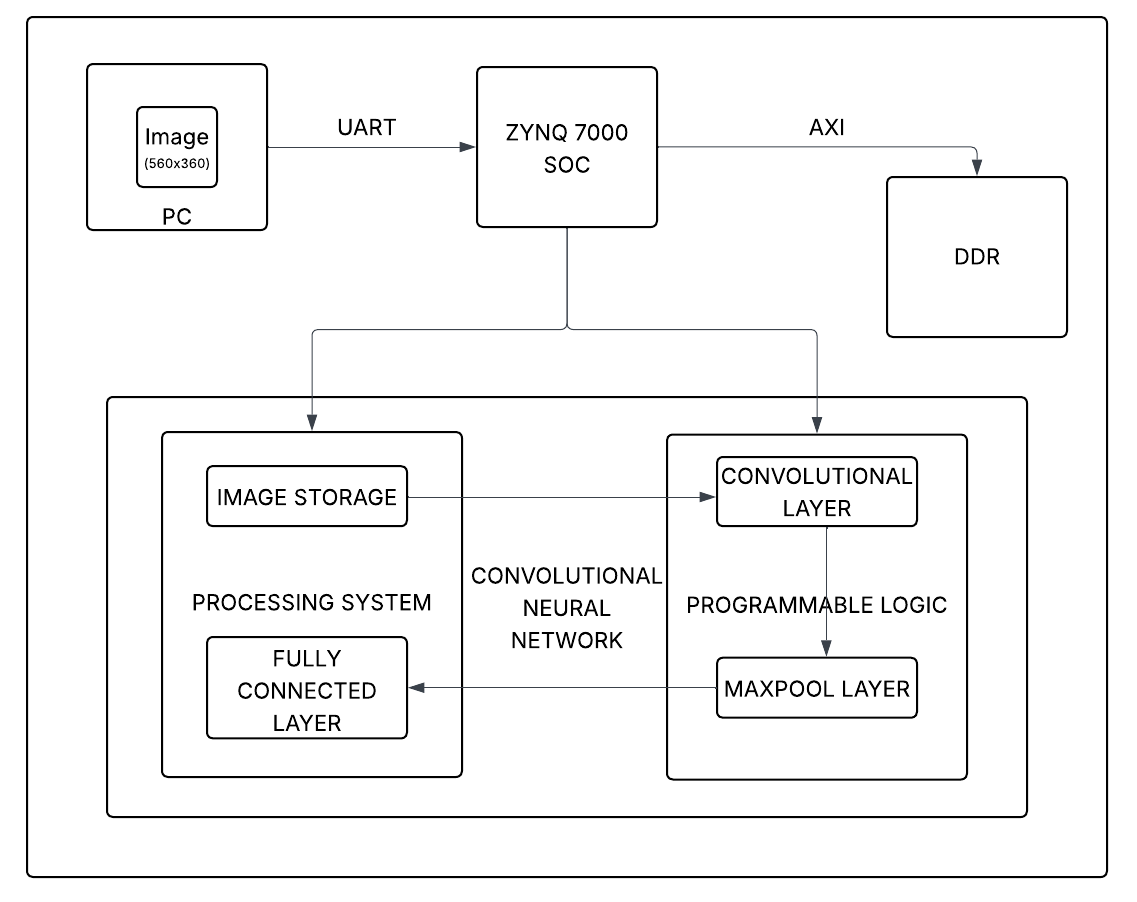
\includegraphics[width=0.8\linewidth]{images/diag_final.png}
        \caption{Hardware software partitioning}
        \label{fig:Hardware Software partitioning}
    \end{figure}
    
    \section{FPGA for Hardware Acceleration}
    \noindent
    The CPU manages diverse tasks efficiently, though it sequentially processes instructions, it has limited capacity for parallel processing and low performance in compute-intensive scenarios. The GPU, or Graphics Processing Unit, is built with many cores optimised for parallel processing. Still, this capability often comes at the cost of higher power consumption, a notable trade-off in its design. The FPGA is composed of a network of CLBs linked through programmable interconnects, thus increasing flexibility through reconfigurability, and could employ parallelism for accelerating operations.

    
    
    \section{Graphical User Interface}
    \noindent
    The FPGA is a very low-level device, it has a lot of peripherals available to it, but to use those peripherals, all of those need to be configured, having configured those interfaces, it is necessary that at the user level, the peripherals must be accessible easily to be able to communicate with the FPGA thus, a GUI needs to be developed. The GUI helps create a proper interface between peripherals and the user.

    \section{Workflow and Timeline}
    
    \subsection{Workflow}
    \begin{figure}[H]
        \centering
        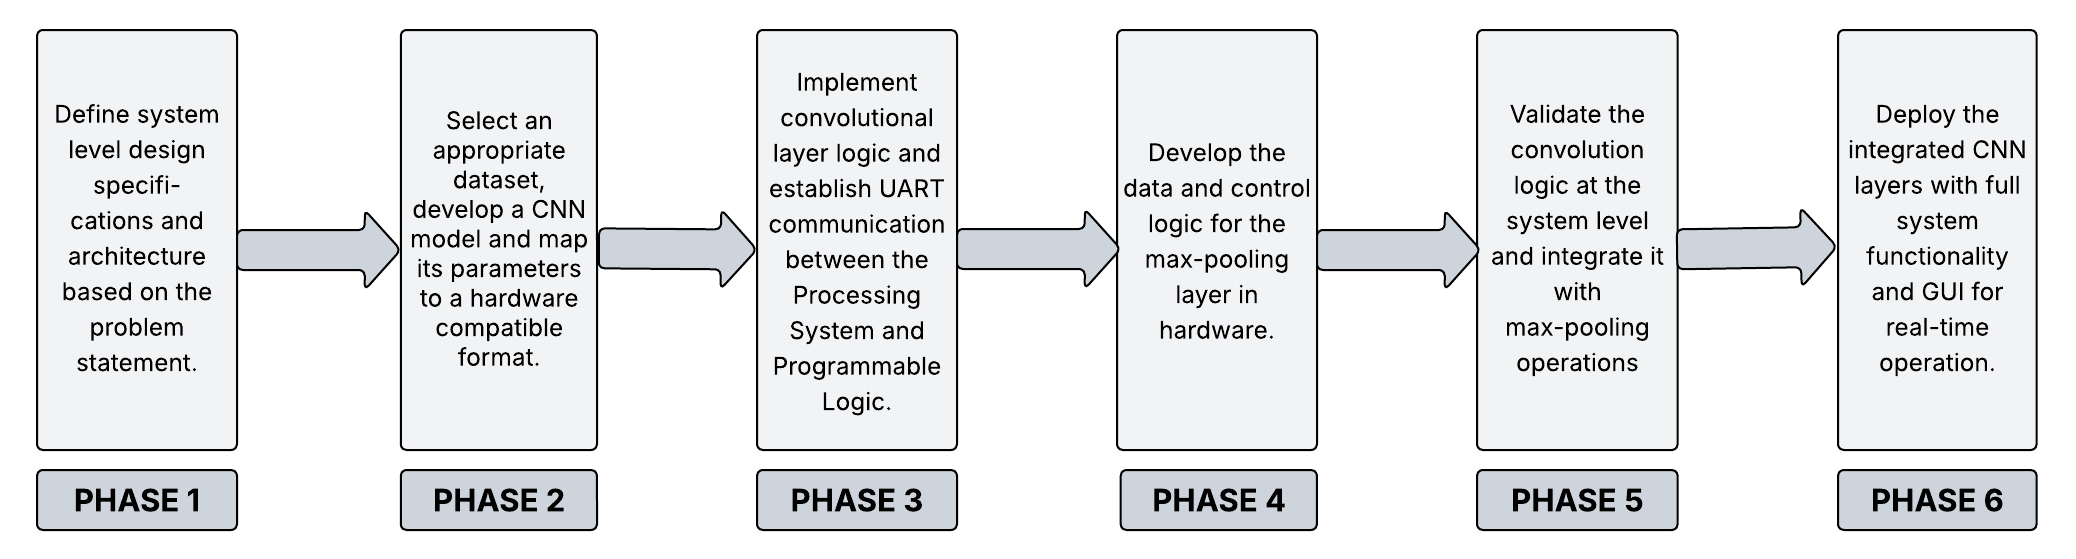
\includegraphics[width=1.1\linewidth]{images/workflow.png}
        \caption{Workflow}
        \label{fig:workflow}
    \end{figure}

    \subsection{Timeline}
    \begin{figure}[H]
        \centering
        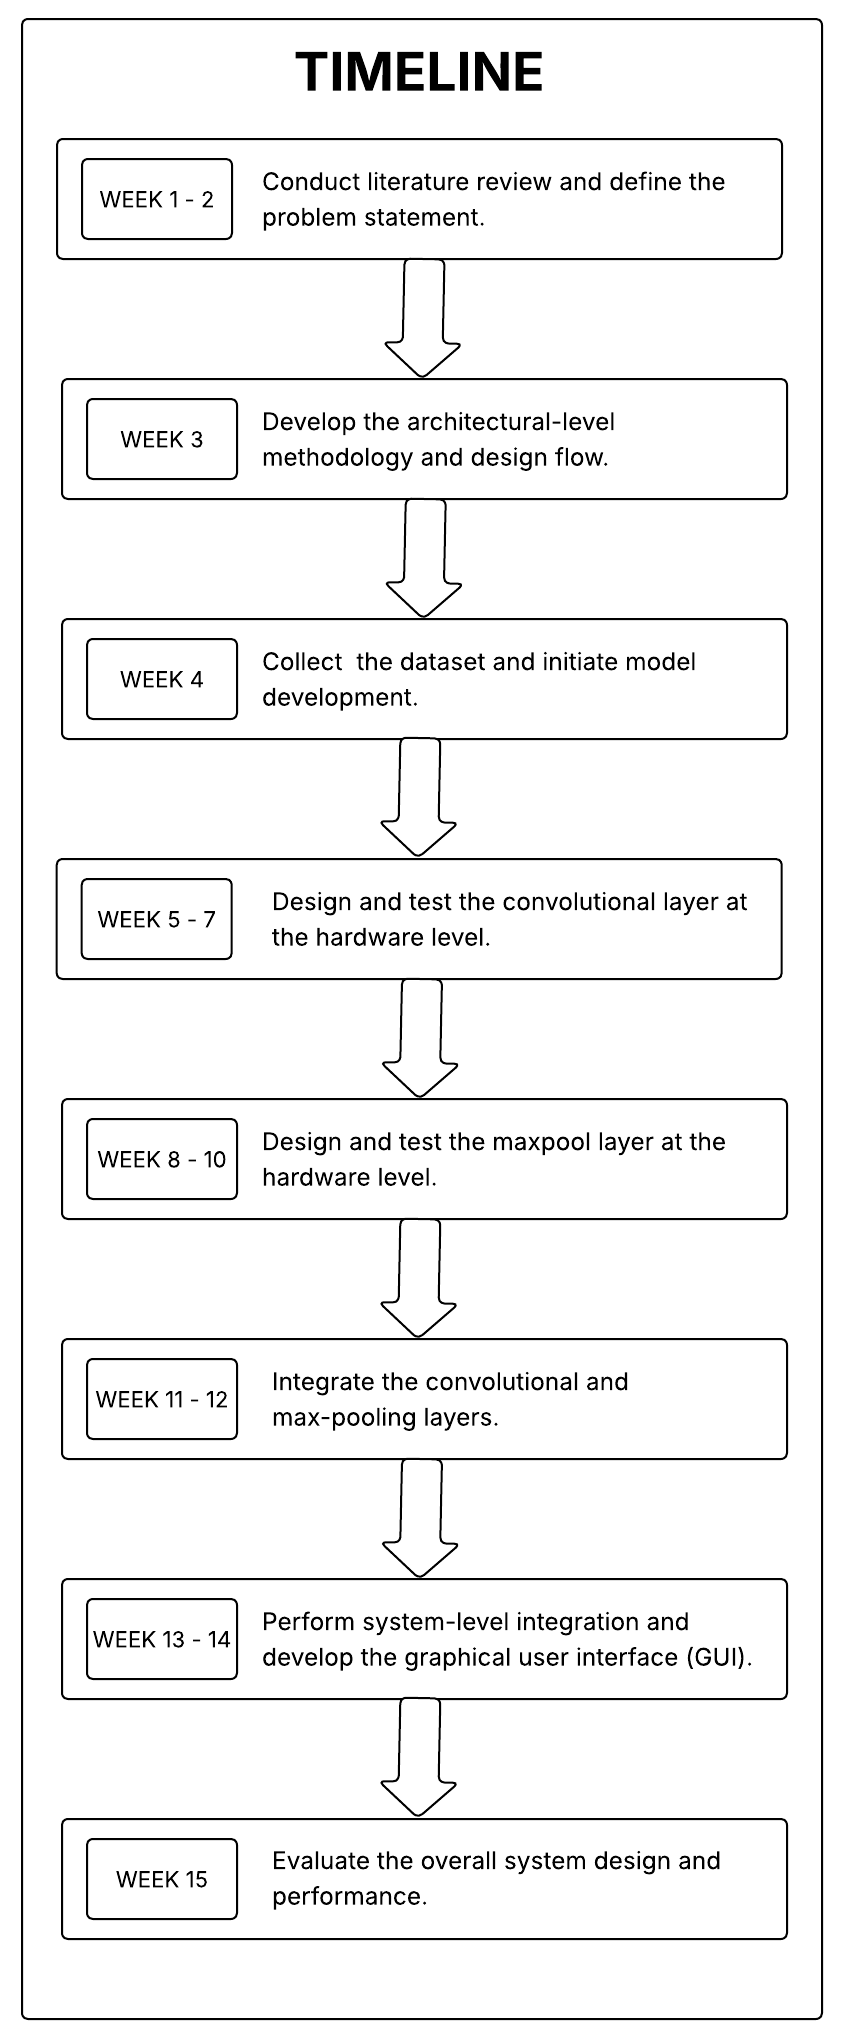
\includegraphics[width=0.57\textwidth]{images/timeline_final.png}
        \caption{Project Timeline}
        \label{fig:timeline}
    \end{figure}
    \newpage
    
    
    
    



    
    

